
\chapter{Introduction}
 
 {\slshape \scshape ``You have to be in a state of play to design. If you're not in a state of play, you can't build anything." - Paula Scher}

Mechatronics is an amalgam of ``mechanisms" and ``electronics": systems that contain both mechanical and electrical components. It's a field that spans nearly every industry, so any one source (even this one) will not be complete with all the information you need. But this may be a good jumping off point. I'm writing this generally towards those in a competitive robotics environment, so will use many examples from there, but you soon find that those same technologies that shoot foam balls into goals can be used anywhere from assembly lines to emergency medical equipment or racecars.

This document is not intended to be all-encompassing. In reality, it's just an outline; a map. We live in an era where information is readily available on demand. This document really doesn't contain anything new. Its goal is to show you a plethora of things that exist in a breadth-first fashion before you dive down a particular rabbit hole. There are a few places where I'll dive deeper because I feel it's relevant to show you some of the nuances you should be aware of. By and large, my goal isn't to drill home every single thing because I'll fail at that and fail you in the process. Someone will come up with something new, or improve something discussed here, and this information will become outdated. I'll try to keep it up to date... but I will definitely fail!

This is partly why I've open-sourced this \LaTeX document. It's not a wiki, because the linearity of a text enables the reader to know they've completed it, and this is more printable. I'd love it if the graphics were more unified, and I appreciate any contributions you might have while preventing this from becoming too big to be useful (as I fear it already is).

Some sections of this will be dry... The human mind is a weird thing. It's better at prompted recall than unprompted recall. You may not always be thinking about the many different types of bolts, but if you've seen one before, and you come across a problem that needs it, you might be able to figure it out - or at least know where to start looking.

I hope to keep this terse. We're going to go fast and I'm going to leave some things to your imagination or research to figure out exactly how they work. I love mechatronics and hope you do too, so I don't want to spoil it by chewing your steak for you.

\addvspace{2.0ex}
\begin{qbox}
	Somtimes you'll see boxes like these which will ask questions or prompt research. The answers won't be in this text! It shouldn't be critical for you to know, either, but if you are so inclined, do some additional research and you'll learn more.
\end{qbox}

With that... let's begin.

\chapter{Physics \& Terminology}
 
 {\slshape \scshape ``I learned very early the difference between knowing the name of something and knowing something." - Richard Feynman}

 Engineers use a lot of nomenclature. While some nomenclature is windowdressing, most of it in engineering is useful in saying exactly what you mean. If you've been through physics, or hung around engineers enough, most of these terms should be self-explanatory. Gloss over this section and use it like a glossary if you come across a word you don't know.

\section{Stresses and Deformations}
We use these terms to denote the shape of material deformation (indicated by the dashed lines and solid shapes), or the direction which a load is applied (indicated by the arrows).
\begin{figure}[H]
\begin{subfigure}[b]{.32\linewidth}
	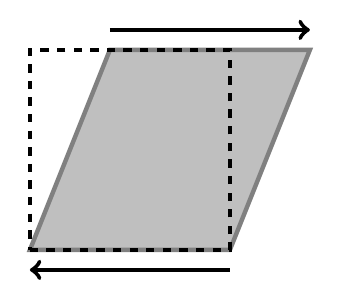
\begin{tikzpicture}[x=1.0in, y=1.0in]
	  %\fill[lightgray] (1.0,0)--(0,1.0)--(0,0)--cycle;
	  \filldraw[color=gray, fill=lightgray, ultra thick] (0,0) -- (1,0) -- (1.4,1) -- (0.4,1) -- cycle;
	  \draw[black, ultra thick, dashed] (0,0) -- (1,0) -- (1.0,1) -- (0.0,1) -- cycle;
	  \draw[black, ->, ultra thick] (1,-0.1) -- (0,-0.1);
	  \draw[black, ->, ultra thick] (0.4,1.1) -- (1.4,1.1);
	\end{tikzpicture}
	\caption{Shear}
\end{subfigure}\begin{subfigure}[b]{.32\linewidth}
	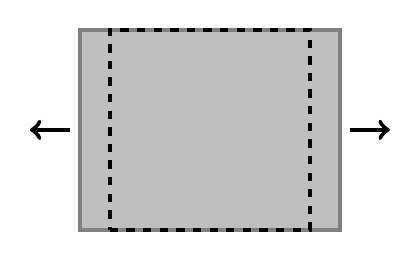
\begin{tikzpicture}[x=1.0in, y=1.0in]
	  %\fill[lightgray] (1.0,0)--(0,1.0)--(0,0)--cycle;
	  \filldraw[color=gray, fill=lightgray, ultra thick] (-0.15,0) -- (1.15,0) -- (1.15,1) -- (-0.15,1) -- cycle;
	  \draw[black, ultra thick, dashed] (0,0) -- (1,0) -- (1.0,1) -- (0.0,1) -- cycle;
	  \draw[black, ->, ultra thick] (-0.2,0.5) -- (-0.4,0.5);
	  \draw[black, ->, ultra thick] (1.2,0.5) -- (1.4,0.5);
	  \draw[black, ->, ultra thick, opacity=0] (1,-0.1) -- (0,-0.1);
	\end{tikzpicture}
	\caption{Axial / Tension}
\end{subfigure}\begin{subfigure}[b]{.32\linewidth}
	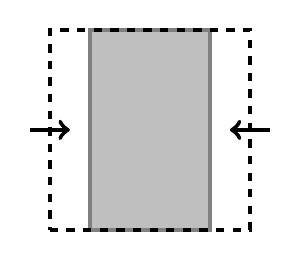
\begin{tikzpicture}[x=1.0in, y=1.0in]
	  %\fill[lightgray] (1.0,0)--(0,1.0)--(0,0)--cycle;
	  \filldraw[color=gray, fill=lightgray, ultra thick] (0.2,0) -- (0.8,0) -- (0.8,1) -- (0.2,1) -- cycle;
	  \draw[black, ultra thick, dashed] (0,0) -- (1,0) -- (1.0,1) -- (0.0,1) -- cycle;
	  \draw[black, <-, ultra thick] (0.1,0.5) -- (-0.1,0.5);
	  \draw[black, <-, ultra thick] (0.9,0.5) -- (1.1,0.5);
	  \draw[black, ->, ultra thick, opacity=0] (1,-0.1) -- (0,-0.1);
	\end{tikzpicture}
	\caption{Axial / Compression}
\end{subfigure}

\begin{subfigure}[b]{.47\linewidth}
	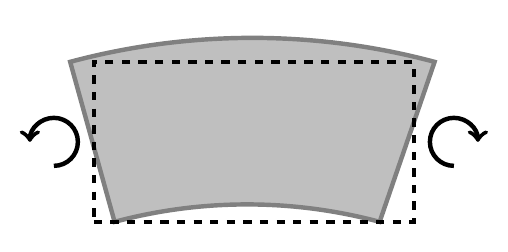
\begin{tikzpicture}[x=0.8in, y=0.8in]
	  %\fill[lightgray] (1.0,0)--(0,1.0)--(0,0)--cycle;
	  \filldraw[color=gray, fill=lightgray, ultra thick] ({0.5*sin(15)},-0.5) arc(105:75:3.2) -- ({2+0.5*sin(15)},0.5) arc(75:105:4.4) -- cycle;
	  \draw[black, ultra thick, dashed] (0,-0.5) -- (2,-0.5) -- (2,0.5) -- (0,0.5) -- cycle;
	  \draw[black, <-, ultra thick] (-0.4,0) arc(180:-90:0.15);
	  \draw[black, <-, ultra thick] (2.4,0) arc(0:270:0.15);
	\end{tikzpicture}
	\caption{Bending}
\end{subfigure}\begin{subfigure}[b]{.47\linewidth}
	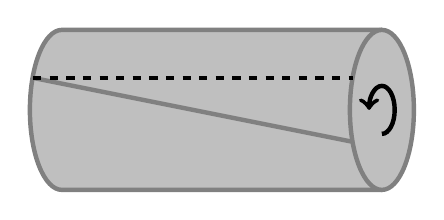
\begin{tikzpicture}[x=0.8in, y=0.8in]
	  \filldraw[color=gray, fill=lightgray, ultra thick] (2,-0.5) -- (0,-0.5) arc (270:90:0.2 and 0.5) -- (2,0.5);
	  \filldraw[color=gray, fill=lightgray, ultra thick] (2,0) circle[x radius=0.2, y radius=0.5];
	  \draw[color=gray, ultra thick] (-0.18, 0.2) -- (1.82, -0.2);
	  \draw[color=black, ultra thick, dashed] (-0.18, 0.2) -- (1.82, 0.2);
	  %\draw[black, <-, ultra thick] (-0.3,0) arc(0:270:0.08 and 0.15);
	  \draw[black, <-, ultra thick] (1.92,0) arc(180:-90:0.08 and 0.15);
	\end{tikzpicture}
	\caption{Torsion}
\end{subfigure}

\begin{subfigure}[b]{.95\linewidth}
	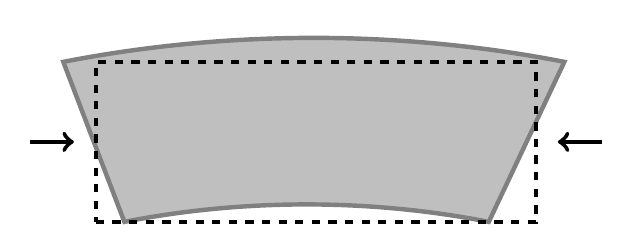
\begin{tikzpicture}[x=1.1in, y=0.8in]
	  %\fill[lightgray] (1.0,0)--(0,1.0)--(0,0)--cycle;
	  \filldraw[color=gray, fill=lightgray, ultra thick] ({0.5*sin(15)},-0.5) arc(105:75:3.2) -- ({2+0.5*sin(15)},0.5) arc(75:105:4.4) -- cycle;
	  \draw[black, ultra thick, dashed] (0,-0.5) -- (2,-0.5) -- (2,0.5) -- (0,0.5) -- cycle;
	  \draw[black, <-, ultra thick] (-0.1,0) -- (-0.3,0);
	  \draw[black, <-, ultra thick] (2.1,0) -- (2.3,0);
	\end{tikzpicture}
	\caption{Buckling}
\end{subfigure}

\end{figure}

\begin{asparaenum}[a)]
	\item \textit{Shear} is two surfaces sliding past each other, sometimes referred to as \textit{parallelogramming} \index{stress!shear}
	\item \textit{Tension} is a form of \textit{axial} stress where material is being pulled apart. \index{stress!tension} \index{stress!axial}
	\item \textit{Compression} is a form of \textit{axial} stress where material is being pushed together. \index{stress!compression}
	\item \textit{Bending} is when a material bows with curvature. \textit{Cupping}, \textit{bowing}, and \textit{crooking} refer to this phenomenon about different axes of a board. \index{stress!bending}
	\item \textit{Torsion} is when material twists along an axis. \index{stress!torsion}
	\item \textit{Buckling} is bending that is induced by compressive loads.
\end{asparaenum}

\section{Directions and Coordinate Systems}
\begin{figure}[H]
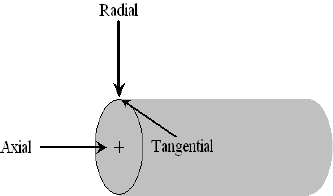
\includegraphics[width=0.45\textwidth]{imgs/cylindrical_coords.png}
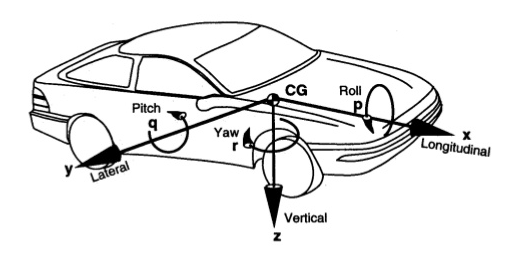
\includegraphics[width=0.45\textwidth]{imgs/sae_coords.png}
\caption{Cylindrical, and Cartesian Coordinates}
\end{figure}

\begin{asparaenum}[a)]
	\item The \textit{axial} direction is along the axis of symmetry for a shaft, or along the axis of rotation for a rotating component. \index{direction!axial}
	\item The \textit{radial} direction(s) are perpindicular to this axis of symmetry, and coincide at a point, emanating outwards. \index{direction!radial}
	\item The \textit{tangential} direction(s) are perpindicular to both the radial and axial directions, curving around the axis of rotation. \index{direction!tangential}
	\item For vehicles, the \textit{longitudinal} direction is along the axis that the vehicle primarially moves forwards and backwards.
	\item For vehicles, the \textit{lateral} axis is left or right.
	\item For vehicles, the \textit{vertical}, or \textit{normal} axis is up-down.
	\item \textit{Roll} is rotation about the longitudinal axis.
	\item \textit{Pitch} is rotation about the lateral axis.
	\item \textit{Yaw} is rotation about the vertical axis.
\end{asparaenum}

Engineers also use a little bit of jargon to refer to different geometric relationships that go beyond your typical geometry class.

\begin{asparaenum}[a)]
	\item \textit{Orthogonal} is a synonym for \textit{perpindicular}; at 90 degrees to. \index{direction!orthogonal}
	\item An axis may be \textit{normal} to a plane if it is perpindicular in two directions. \index{direction!normal}
	If the plane and axis have specified positive directions, it may be \textit{antinormal} if the positive directions are opposed to each other. \index{direction!antinormal}
	\item Axes and planes may be \textit{parallel} to each other. \index{direction!parallel}
	\item Axes and planes may be \textit{antiparallel} to each other if the positive directions are opposed to each other. \index{direction!antiparallel}
	\item A surface (with nonzero curvature) can be \textit{tangent} to a line or another surface if they are coincident at a point or path which is not a sharp corner. \index{direction!tangent}
\end{asparaenum}

\section{Basic Dynamics}

\begin{asparaenum}[a)]
	\item \textit{Mass} ($m$) is the amount of matter an object has.
	\item \textit{Force} ($F$) is motive for objects to change velocity.
	\item \textit{Acceleration} ($a$) is a change in an object's velocity over time.
	\textit{Velocity} ($v$) is a change in an object's position over time.
	\textit{Position} ($x$) is an object's location in space.
\end{asparaenum}

These three ideas are summed up in the equation of

\begin{align}
	\vec{F_{net}} = m \times \vec{a}
\end{align}
\index{Newton's law}

(for rigid objects which do not change mass). You may ask why the $\vec{F}$ and $\vec{a}$ have that little arrow over the top of them. That's to denote that they are \textit{vectors}; they have multiple components. You can break this equation down simply into

\begin{align}
	F_x = m \times a_x \\
	F_y = m \times a_y \\
	F_z = m \times a_z
\end{align}

These concepts exist in an analogue for rotating components as well.
\begin{asparaenum}[a)]
	\item \textit{Moment of inertia} or \textit{MOI} ($I$) is a measure of how spread out an object's mass is. A point mass (black hole) has a MOI of zero. A golf ball would have a small MOI, and a beach ball would have a large MOI, even if the beach ball has less mass.
	\item \textit{Torques} or \textit{moments} ($T$ or $M$) are twisting forces. They can be quantified by how much force is applied multiplied by the lever arm which it is applied by.
	\item \textit{Angular acceleration, velocity, and positions} ($\alpha$, $\omega$, $\theta$) are just like their linear counterparts, except they are measured as rotation about an axis.
\end{asparaenum}

\begin{align}
	\vec{M} = \frac{d}{dt} [I] \vec{\omega}
\end{align}

(which again holds for rigid objects). You may ask why the moment of inertia $[I]$ has those brackets around it. That's to denote that it's a \textit{matrix}. This means that breaking the equation down is difficult if there are multiple rotations. The $\frac{d}{dt}$ is a derivative, a concept from calculus which represents change over time. Luckily, for the simple case of an object of constant moment of inertia, and spinning only about one axis $x$,

\begin{align}
	M_x = I_x \alpha_x
\end{align}

which isn't so scary, and is just like the linear case.

\textit{Energy} is a property that can be transformed in many ways to do useful \textit{work}. There are many forms of energy (spring, gravitational, electrical, chemical) and many different processes that can be used to transform it (combustion, releasing a spring, lifting a heavy object).
\textit{Power} is a measure of energy transformation / transfer per unit time.

Congratulations! You've just learned the basics to 80\% of newtonian physics.

\section{Basic Electronics}
There are a few basic electrical terms which can be confusing at first since they are not everyday, lived phenomena.

\begin{asparaenum}[a)]
	\item \textit{Current} $I$ (measured in \textit{Amperes}, or amps, $A$) is (roughly) a measure of how many electrons pass through a cross-sectional area (e.g. a wire) per second.
	\item \textit{Voltage} $V$ or \textit{Electric Potential} (measured in \textit{Volts}, $V$) is a measure of the motive force that is available to push electrons. It is always a relative measurement taken between two points. If it is given as a plain number (e.g. ``this terminal has 12 volts"), then there must be an assumed \textit{ground} that the measurement is taken from.
	\item \textit{Resistance} $R$ (measured in \textit{Ohms}, $\Omega$) is a measure of how much voltage is required to get a certain amount of current to flow though. Ohm's law expresses this as $\Delta V = I \times R$; the voltage drop across a wire is proportional to both the current passing through it and its resistance. Resistance of a wire can be reduced by using a superior material (copper rather than aluminum), using a larger cross-section (or wire \textit{gague}), and shortening the wire.
\end{asparaenum}

These concepts are often related to hydraulic systems; voltage is much like pressure, and current like flow rate.

This also leads us to a few laws known as \textit{Kirchoff's laws}.

Kirchoff's Voltage Law states that ``the sum of the voltages across all components in a loop add up to zero". Mathematically,
\begin{align}
	\sum_{loop} \Delta V = 0
\end{align}

Some thinking would reveal that this is merely a different way of stating that ``all voltages are relative."

Kirchoff's Current Law states that ``the sum of currents entering a node (a point where multiple components meet) add up to zero". Mathematically,
\begin{align}
	\sum_{node} I = 0
\end{align}

This should make sense as the electrons must go somewhere. This is merely a different way of stating that ``electrons cannot be destroyed."